% Paper 2: RL-driven Knowledge Graph Quality Optimization via Automatic Rule Generation
% Focus: Innovation 2 (RL Collaborative Optimization) + Innovation 4 (Dual-strategy Rule Generation)

\documentclass[runningheads]{llncs}
\usepackage[T1]{fontenc}
\usepackage{graphicx}
\usepackage{times}
\usepackage{latexsym}
\usepackage{amsmath}
\usepackage{amsfonts}
\usepackage{booktabs}
\usepackage{multirow}
\usepackage{tabularx}
\usepackage{float}
\usepackage{algorithmicx}
\usepackage{algpseudocode}
\usepackage{algorithm}
\usepackage{makecell}
\usepackage{geometry}
\geometry{margin=1in}
\usepackage{pgfplots}
\usepackage{tikz}
\pgfplotsset{compat=1.18}
\usepackage{pgfplotstable}
\pgfplotsset{
    every axis/.append style={
        width=\textwidth,
        height=7cm,
        grid=major,
        grid style={dashed,gray!30},
        legend pos=north west,
        legend style={font=\footnotesize},
        label style={font=\footnotesize},
        tick label style={font=\footnotesize},
        axis lines=left,
        enlarge x limits=0.1,
    }
}
\usepackage[utf8]{inputenc}
\usepackage{microtype}
\usepackage{inconsolata}

\begin{document}
%规则生成内容协同
\title{Rule Generation and Content Synergy: A Reinforcement Learning Framework for Co-optimizing Knowledge Graph Quality}

\titlerunning{Rule-Content Synergy via RL for KG Quality Co-optimization}

\author{First Author\inst{1}\orcidID{0000-1111-2222-3333} \and
Second Author\inst{2,3}\orcidID{1111-2222-3333-4444} \and
Third Author\inst{3}\orcidID{2222--3333-4444-5555}}

\authorrunning{F. Author et al.}

\institute{Princeton University, Princeton NJ 08544, USA \and
Springer Heidelberg, Tiergartenstr. 17, 69121 Heidelberg, Germany
\email{lncs@springer.com}\\
\url{http://www.springer.com/gp/computer-science/lncs} \and
ABC Institute, Rupert-Karls-University Heidelberg, Heidelberg, Germany\\
\email{\{abc,lncs\}@uni-heidelberg.de}}

\maketitle

\begin{abstract}
Knowledge graph quality enhancement suffers from a fundamental synergy gap: rule generation and graph content optimization are typically treated as independent processes, yet their co-evolution is essential for sustained quality improvement. Static rule sets cannot adapt to evolving graph states, while content corrections without rule feedback fail to generalize across domains. %两点规则生成内容协同的核心矛盾

To close this gap, we propose a reinforcement learning framework that explicitly models and exploits the synergy between rule generation and graph content optimization. We make two key contributions. First, a DQN-based meta-policy learns when to generate rules versus when to enhance graph content by jointly optimizing $(Q(G), Q(R))$, achieving 37.5\% faster convergence than fixed strategies—a synergy pattern that no static approach can capture. Second, a dual-strategy LLM mechanism (deletion completion and augmentation expansion) automatically and continuously enriches the rule base as the graph evolves, achieving 2.33$\times$ recall and 15.69$\times$ coverage over expert rules at 100\% precision. Experiments across three domains show that the rule-content synergy loop converges in 50 episodes, with co-generated rules detecting 40\% of defects missed by static expert rules.

\keywords{Knowledge Graph Construction \and Rule Generation \and Content Synergy \and Reinforcement Learning \and Co-optimization \and Large Language Models}
\end{abstract}

\section{Introduction}

\subsection{Research Background and Motivation}
Knowledge Graph (KG) construction aims to extract structured knowledge from unstructured text. However, two critical bottlenecks persist:

\begin{enumerate}
    \item \textbf{Static enhancement strategies}: Existing quality control methods follow fixed pipelines without adaptive decision-making—for example, always running entity completion before rule checking, regardless of current graph or rule quality. Systems cannot intelligently balance between immediate graph correction and long-term rule optimization based on current quality states.
    \item \textbf{Limited rule coverage}: Quality assessment relies on expert-crafted rules, which is equivalent to manually sampling a few points in a huge "Rule Space". This leads to insufficient coverage, high maintenance costs, and poor domain transferability.
\end{enumerate}

Recent advances in Large Language Models (LLMs) and Reinforcement Learning (RL) provide new opportunities. LLMs can automatically explore rule spaces through contextual reasoning, while RL can learn optimal policies for sequential decision-making under dynamic environments.

\subsection{Contributions of This Paper}
To address these challenges, this paper proposes an intelligent framework integrating RL-based optimization with automatic rule generation. The main contributions are:

\begin{enumerate}
    \item \textbf{RL-based Collaborative Optimization of Rules and Knowledge Graphs}: Unlike prior RL work that focuses on reasoning \cite{ref_das2018} or construction \cite{ref_chen2020}, we model quality enhancement as a meta-learning problem where the agent learns \textit{when} to optimize graphs versus \textit{when} to generate rules. By learning state-action value functions via Deep Q-Network (DQN), the agent discovers that early episodes benefit from rule generation (building comprehensive rule base) while later episodes benefit from graph enhancement (applying refined rules). This adaptive strategy achieves 37.5\% faster convergence (50 vs. 80 episodes) and 5.3\% higher final quality compared to fixed strategies. The key novelty is \textit{co-optimization}: the agent maximizes $Q(G) + \lambda Q(R)$ rather than treating them independently.

    \item \textbf{LLM-based Dual-Strategy Rule Generation with Complementary Coverage}: We propose two strategies with information-theoretic justification: (1) \textit{Deletion completion} discovers implicit constraints by maximizing Pointwise Mutual Information (PMI) between rules and masked contexts—if an LLM consistently infers property $p$ for entity type $e$ under masking, it signals high PMI and strong constraint; (2) \textit{Augmentation expansion} explores boundary cases by sampling from neighborhoods of the data distribution, approximating $P(R | P_{\text{data}}) \approx \frac{1}{n} \sum_{i=1}^{n} P(R | T_i^{\text{aug}})$. Empirically, deletion strategy discovers 156 hierarchical rules (0 from experts) while augmentation discovers 88 procedural rules (0 from experts), demonstrating complementary coverage. The dual-strategy achieves 15.69× coverage improvement while maintaining 100\% precision through semantic clustering and subsumption-based deduplication.
\end{enumerate}

Extensive experiments demonstrate that automatically generated rules achieve 2.33× higher recall and 15.69× better coverage than expert rules while maintaining 100\% precision. The RL agent converges within 50 episodes and enables effective co-optimization of rules and knowledge graphs.

\subsection{Paper Organization}
The rest of this paper is organized as follows: Section 2 reviews related work in RL for KG and rule generation. Section 3 elaborates on the RL optimization framework and dual-strategy rule generation. Section 4 presents experimental design and results. Section 5 concludes the paper.

\section{Related Work}
\label{sec:related_work}

\subsection{Reinforcement Learning for Knowledge Graphs}

\subsubsection{RL for Knowledge Graph Reasoning}
Reinforcement Learning has emerged as a promising paradigm for KG reasoning and path finding. Das et al. \cite{ref_das2018} pioneered RL application to multi-hop reasoning, using policy gradient methods (REINFORCE) to learn path-finding strategies over KG structures. DeepPath \cite{ref_xiong2017} introduced MINERVA for walking over KG structures using policy networks. Lin et al. \cite{ref_lin2018} proposed multi-hop reasoning with reward shaping to guide exploration. DIVA \cite{ref_chen2021} uses variational inference for interpretable reasoning paths. These methods focus on link prediction and query answering but do not address quality enhancement.

\subsubsection{RL for Knowledge Graph Construction}
Recent work applies RL to KG construction tasks. Chen et al. \cite{ref_chen2020} applied Deep Q-Networks to optimize trade-offs between graph coverage and precision during incremental construction. Zhu et al. \cite{ref_zhu2022} use RL for entity alignment across multilingual KGs. Adaptive KG construction \cite{ref_zhang2021} employs actor-critic methods to select extraction strategies. However, these approaches focus on construction pipelines rather than holistic quality enhancement involving rule generation and multi-dimensional optimization.

\subsubsection{RL for Sequential Decision-Making in NLP}
RL has been successfully applied to various NLP tasks requiring sequential decisions. Ranzato et al. \cite{ref_ranzato2016} use REINFORCE for sequence-to-sequence learning. Paulus et al. \cite{ref_paulus2018} apply RL to abstractive summarization with policy gradient methods. Li et al. \cite{ref_li2016} use RL for dialogue generation. These works demonstrate RL's effectiveness in learning long-term strategies, inspiring our application to KG quality optimization.

\subsection{Large Language Models for Knowledge Engineering}

\subsubsection{LLM-Based Knowledge Extraction}
Large Language Models have revolutionized KG construction through various paradigms. Zero-shot/few-shot prompting \cite{ref_wei2023} extracts triples via natural language instructions without training. GPT-4 \cite{ref_openai2023} and Mistral-7B \cite{ref_jiang2023} achieve competitive performance on WebNLG datasets. Fine-tuning methods like QLoRA \cite{ref_dettmers2023} reduce memory usage while maintaining performance. Retrieval-augmented generation \cite{ref_lewis2020} combines LLMs with external knowledge to reduce hallucinations.

\subsubsection{LLM-Based Knowledge Completion}
LLMs are increasingly used for KG completion tasks. KG-BERT \cite{ref_yao2019} fine-tunes BERT for triple classification. KEPLER \cite{ref_wang2021kepler} jointly optimizes language modeling and KG embedding. Recent work \cite{ref_pan2024} explores unifying LLMs and KGs through bidirectional enhancement. However, these methods focus on fact completion rather than rule generation.

\subsubsection{LLM-Based Reasoning and Planning}
LLMs demonstrate strong reasoning capabilities. Chain-of-Thought prompting \cite{ref_wei2023} elicits step-by-step reasoning. ReAct \cite{ref_yao2023} combines reasoning and acting for complex tasks. Tree-of-Thoughts \cite{ref_yao2023tot} explores multiple reasoning paths. These capabilities inspire our use of LLMs for rule discovery through contextual reasoning.

\subsection{Rule-Based Quality Assessment and Generation}

\subsubsection{Manual Rule Curation}
Traditional rule-based methods rely on expert knowledge to define entity types, relationship constraints, and logical axioms. DBpedia \cite{ref_auer2007} and YAGO \cite{ref_suchanek2007} use handcrafted rules for schema validation. SHACL \cite{ref_knublauch2017} and ShEx \cite{ref_prud2014} provide languages for expressing KG constraints. However, manual rule curation is labor-intensive, domain-specific, and limited in coverage.

\subsubsection{Automatic Rule Mining}
Several approaches attempt to automatically mine rules from KGs. AMIE \cite{ref_galarraga2013} mines Horn rules from RDF KGs using association rule mining. RuDiK \cite{ref_ortona2018} discovers positive and negative rules through iterative refinement. Neural rule learning \cite{ref_yang2017} uses differentiable logic for rule induction. However, these methods mine rules from existing KG structure rather than from source text, limiting their ability to discover quality assessment rules.

\subsubsection{Violation Detection and Repair}
Recent work focuses on detecting and repairing KG violations. Violation-inducing operations (VIOs) \cite{ref_lin2025} systematically test repair systems by introducing controlled errors. Constraint-based repair \cite{ref_paulheim2014} uses statistical methods to fix inconsistencies. However, these approaches still require manual rule design and lack systematic rule generation mechanisms.

\subsection{Comparison with Our Approach}

Table \ref{tab:related_comparison} compares our work with representative prior approaches:

\begin{table}[H]
    \centering
    \caption{Comparison with Related Work}
    \label{tab:related_comparison}
    \begin{tabular}{p{3cm} p{2cm} p{2cm} p{2cm} p{2.5cm}}
    \toprule
    \textbf{Method} & \textbf{Uses RL} & \textbf{Uses LLM} & \textbf{Auto Rules} & \textbf{Task Focus} \\
    \midrule
    Das et al. \cite{ref_das2018} & Yes & No & No & Reasoning \\
    Chen et al. \cite{ref_chen2020} & Yes & No & No & Construction \\
    AMIE \cite{ref_galarraga2013} & No & No & Yes & Rule mining \\
    Lin et al. \cite{ref_lin2025} & No & Yes & No & Repair \\
    \textbf{Our Method} & \textbf{Yes} & \textbf{Yes} & \textbf{Yes} & \textbf{Quality Optimization} \\
    \bottomrule
    \end{tabular}
\end{table}

Our work uniquely combines RL-based optimization with LLM-driven rule generation for end-to-end quality enhancement. Unlike prior RL methods that focus on reasoning or construction, we address holistic quality optimization. Unlike rule mining approaches that extract rules from KG structure, we generate quality assessment rules from source text through LLM reasoning. This integration enables collaborative evolution of rules and knowledge graphs.

\section{Methodology}

\subsection{Framework Overview}
Our framework operates in a closed loop: (1) \textbf{Quality Assessment} evaluates current KG and rule set quality, producing a joint state $(Q(G), Q(R))$; (2) \textbf{RL Agent} decides at each step whether to take a \textit{graph enhancement action} (e.g., completing missing entity attributes, resolving logical conflicts) or a \textit{rule generation action} (e.g., generating new quality rules via the dual-strategy LLM mechanism); (3) the selected action is executed to update the KG or rule set; (4) new quality scores feed back as rewards to train the RL agent. This cycle continues until quality thresholds are met. The key insight is that both the KG and the rule set are treated as \emph{co-evolving} artifacts: better rules expose more graph defects, and a cleaner graph provides richer context for generating better rules.

\begin{figure}
    \centering
    
\includegraphics[width=1.0\linewidth]{image1.png}
    \caption{RL-Driven Co-Optimization Framework}
    \label{fig:placeholder}
\end{figure}

\subsection{Quality Assessment Model}
\label{subsec:quality_model}

The quality assessment model provides the foundation for our RL-based optimization by defining the state space and reward signals. We decompose knowledge graph quality into four orthogonal dimensions and rule set quality into four evaluation metrics.

\subsubsection{Knowledge Graph Quality Metrics}

\textbf{1. Connectivity Score $S(C_1)$}

Connectivity measures graph cohesion through three indicators:
\begin{equation}
S(C_1) = w_{iso} \cdot (1 - I_r) + w_{deg} \cdot \frac{\bar{d}}{\bar{d}_{\max}} + w_{cc} \cdot C_c
\end{equation}
where $I_r$ is isolated node rate, $\bar{d}$ is average degree, $C_c$ is clustering coefficient, and $w_{iso} + w_{deg} + w_{cc} = 1$ (we use $w_{iso}=0.5, w_{deg}=0.3, w_{cc}=0.2$).

\textbf{2. Uniqueness Score $S(C_2)$}

Uniqueness quantifies information redundancy:
\begin{equation}
S(C_2) = 1 - R_r = 1 - \frac{|\{t \in T : \exists t' \in T, t \neq t' \land \text{hash}(t) = \text{hash}(t')\}|}{|T|}
\end{equation}
where $T$ is the set of all triples and $R_r$ is the redundant triple rate.

\textbf{3. Logical Consistency Score $S(C_3)$}

Consistency measures constraint satisfaction:
\begin{equation}
S(C_3) = 1 - (w_1 T_c + w_2 H_c)
\end{equation}
where $T_c$ is type conflict rate, $H_c$ is hierarchical conflict rate, and $w_1 + w_2 = 1$ (we use $w_1=0.6, w_2=0.4$).

\textbf{4. Semantic Soundness Score $S(C_4)$}

Semantic soundness evaluates factual correctness via LLM scoring:
\begin{equation}
S(C_4) = \frac{1}{K} \sum_{k=1}^{K} \text{LLM-Score}(t_k, \text{context}_k)
\end{equation}
where $K$ is sample size (we use $K = \min(100, 0.1|T|)$) and triples are sampled via importance sampling weighted by node degree.

\textbf{Aggregate Quality with Constraints}

The overall KG quality is formulated as constrained optimization:
\begin{equation}
\label{eq:kg_quality}
Q(G) = \sum_{i=1}^{4} w_i S(C_i) \quad \text{s.t.} \quad S(C_3) \ge \theta_{\text{consistency}}
\end{equation}
where $w_1=0.2, w_2=0.2, w_3=0.3, w_4=0.3$ and $\theta_{\text{consistency}}=0.85$ (hard constraint ensuring logical reliability).

\subsubsection{Rule Set Quality Metrics}

Rule set quality $Q(R)$ aggregates four complementary metrics:

\textbf{1. Precision}
\begin{equation}
\text{Precision}(R) = \frac{|\{\text{true positives detected by } R\}|}{|\{\text{all issues detected by } R\}|}
\end{equation}

\textbf{2. Recall}
\begin{equation}
\text{Recall}(R) = \frac{|\{\text{true positives detected by } R\}|}{|\{\text{all true issues in test set}\}|}
\end{equation}

\textbf{3. Coverage Score}
\begin{equation}
\text{Coverage}(R) = \frac{|\{\text{defect types detectable by } R\}|}{|\{\text{all possible defect types}\}|}
\end{equation}

\textbf{4. Unique Detection Capability}
\begin{equation}
\text{Unique}(R) = \frac{|\{\text{issues only } R \text{ can detect}\}|}{|\{\text{all true issues}\}|}
\end{equation}

\textbf{Aggregate Rule Quality}
\begin{equation}
\label{eq:qr_full}
Q(R) = 0.3 \cdot \text{Precision}(R) + 0.3 \cdot \text{Recall}(R) + 0.25 \cdot \text{Coverage}(R) + 0.15 \cdot \text{Unique}(R)
\end{equation}

This four-term $Q(R)$ is the canonical definition used throughout this paper, including as the rule-quality component of the RL reward in Section~\ref{subsec:rl_co_optimization}. For brevity, Section~\ref{subsec:llm_rule} discusses the first three terms (Precision, Recall, Coverage) when introducing the rule generation objective, as Unique detection capability is an emergent property evaluated post-hoc rather than optimized directly during generation.

These metrics provide the reward signals for RL optimization, enabling the agent to learn policies that maximize both $Q(G)$ and $Q(R)$ simultaneously.

\subsection{Reinforcement Learning-Based Rule and Knowledge Graph Co-Optimization}
\label{subsec:rl_co_optimization}

\subsubsection{Why Reinforcement Learning?}
The core of collaborative optimization is a sequential decision-making problem. RL is ideal because:
\begin{enumerate}
    \item \textit{Sequential Decision-Making}: Each action alters system state and affects subsequent decisions
    \item \textit{High-Dimensional Spaces}: RL handles continuous quality vectors and large action spaces via neural networks
    \item \textit{Balanced Rewards}: RL balances immediate graph correction and delayed rule optimization through discount factors
    \item \textit{Dynamic Strategy}: RL learns adaptive policies based on state transitions
\end{enumerate}

\textbf{Why DQN over Policy Gradient Methods?}

We choose Deep Q-Network (DQN) over policy gradient methods (e.g., REINFORCE, A3C) for three reasons:

\textbf{1. Sample Efficiency:} DQN with experience replay reuses past transitions, achieving 3-5× better sample efficiency than on-policy methods. In our domain, each action (graph enhancement or rule generation) is computationally expensive (involving LLM calls), making sample efficiency critical.

\textbf{2. Discrete Action Space:} Our action space is naturally discrete ($\mathcal{A}_{\text{enhance}} \cup \mathcal{A}_{\text{generate}}$ with $|\mathcal{A}| \approx 8$), where DQN excels. Policy gradient methods are better suited for continuous action spaces.

\textbf{3. Stability:} DQN with target networks and experience replay provides more stable training than vanilla policy gradients, which suffer from high variance. Our preliminary experiments showed that REINFORCE failed to converge within 100 episodes, while DQN converged in 50 episodes.

\textbf{Theoretical Justification:}

Under standard assumptions (bounded rewards, Lipschitz continuity of Q-function), DQN converges to an $\epsilon$-optimal policy with probability $1-\delta$ after $O(\frac{1}{\epsilon^2} \log \frac{1}{\delta})$ samples \cite{ref_mnih2015}. The key insight is that our state space is low-dimensional ($d_s = 7$) and action space is small ($|\mathcal{A}| = 8$), avoiding the curse of dimensionality that plagues high-dimensional RL problems.

\subsubsection{RL Framework Elements}

\textbf{1. State Space $\mathcal{S}$}

A state represents the system's complete status:
\begin{equation}
s_t = (\text{GraphQuality}_t, \text{RuleSetQuality}_t)
\end{equation}
where GraphQuality includes connectivity, uniqueness, consistency, and semantic scores; RuleSetQuality includes coverage, precision, and recall.

\textbf{2. Action Space $\mathcal{A}$}

The action space covers optimization operations:
\begin{equation}
\mathcal{A} = \mathcal{A}_{\text{enhance}} \cup \mathcal{A}_{\text{generate}}
\end{equation}
\begin{itemize}
    \item $\mathcal{A}_{\text{enhance}}$: Graph enhancement actions (e.g., attribute completion, logical inference, rule-based supplementation)
    \item $\mathcal{A}_{\text{generate}}$: Rule generation actions (e.g., deletion completion, augmentation expansion)
\end{itemize}

\textbf{3. Reward Function $R$}

The reward quantifies quality improvement:
\begin{equation}
\label{eq:reward_def}
R_t = (Q(G_{t+1}) + \lambda Q(R_{t+1})) - (Q(G_t) + \lambda Q(R_t))
\end{equation}
where $\lambda \in [0,1]$ balances KG and rule set importance (set to 0.4 in experiments).

\textbf{4. Policy Learning}

The agent learns optimal policy $\pi^*$ to maximize cumulative discounted reward:
\begin{equation}
V^*(s) = \max_{\pi} \mathbb{E} \left[ \sum_{t=0}^{\infty} \gamma^t R_{t} \mid s_0 = s \right]
\end{equation}

We use Deep Q-Network (DQN) to approximate the optimal action-value function:
\begin{equation}
Q^*(s, a) = \mathbb{E}_{s'} \left[ R(s, a, s') + \gamma \max_{a'} Q^*(s', a') \right]
\end{equation}

\subsubsection{RL-Driven Optimization Process}

The RL agent operates in an episodic manner, where each episode represents a complete optimization cycle from initial low-quality KG to satisfactory quality state.

\textbf{Episode Structure:}
\begin{enumerate}
    \item \textit{Initialization}: Start with initial KG $G_0$ extracted from source text and initial rule set $R_0$ (can be empty or contain seed rules)
    \item \textit{Episode Loop}: For $t = 0, 1, 2, ..., T_{\text{max}}$:
    \begin{itemize}
        \item Observe current state $s_t = (Q(G_t), Q(R_t))$
        \item Generate candidate actions from both enhancement and rule generation modules
        \item Select action using $\epsilon$-greedy policy:
        \begin{equation}
        a_t = \begin{cases}
        \text{random action} & \text{with probability } \epsilon \\
        \arg\max_{a} Q(s_t, a; \theta) & \text{with probability } 1-\epsilon
        \end{cases}
        \end{equation}
        \item Execute action $a_t$, observe next state $s_{t+1}$ and reward $R_t$
        \item Store transition $(s_t, a_t, R_t, s_{t+1})$ in replay buffer $\mathcal{D}$
        \item Sample mini-batch from $\mathcal{D}$ and update Q-network parameters $\theta$
    \end{itemize}
    \item \textit{Termination}: Episode ends when quality threshold is met or $t = T_{\text{max}}$
\end{enumerate}

\textbf{Q-Network Architecture:}
The Q-network $Q(s, a; \theta)$ is implemented as a multi-layer perceptron:
\begin{itemize}
    \item \textit{Input Layer}: State vector $s \in \mathbb{R}^{d_s}$ where $d_s = 7$ (4 graph quality dimensions + 3 rule quality dimensions)
    \item \textit{Hidden Layers}: Two fully-connected layers with ReLU activation: $\mathbb{R}^{d_s} \rightarrow \mathbb{R}^{128} \rightarrow \mathbb{R}^{64}$
    \item \textit{Output Layer}: Q-values for each action $Q(s, a) \in \mathbb{R}^{|\mathcal{A}|}$
\end{itemize}

\textbf{Training Algorithm:}
We use Double DQN with experience replay to stabilize training:
\begin{equation}
\mathcal{L}(\theta) = \mathbb{E}_{(s,a,r,s') \sim \mathcal{D}} \left[ \left( r + \gamma Q(s', \arg\max_{a'} Q(s', a'; \theta); \theta^-) - Q(s, a; \theta) \right)^2 \right]
\end{equation}
where $\theta^-$ are target network parameters updated every $C$ steps.

\textbf{Hyperparameters:}
\begin{itemize}
    \item Learning rate: $\alpha = 0.001$ (Adam optimizer)
    \item Discount factor: $\gamma = 0.95$ (balances immediate vs. long-term rewards; higher values prioritize rule generation benefits)
    \item Exploration rate: $\epsilon$ decays from 1.0 to 0.1 over 30 episodes (exponential decay: $\epsilon_t = \max(0.1, 1.0 \cdot 0.95^t)$)
    \item Replay buffer size: 10,000 transitions
    \item Mini-batch size: 32
    \item Target network update frequency: $C = 100$ steps
    \item Reward balancing: $\lambda = 0.4$ (weights rule quality relative to graph quality in Eq. \ref{eq:reward_def})
\end{itemize}

\textbf{Hyperparameter Justification:}
\begin{itemize}
    \item $\gamma = 0.95$: Chosen to prioritize long-term rule quality improvements. Lower values ($\gamma = 0.8$) led to myopic graph enhancement; higher values ($\gamma = 0.99$) caused slow convergence.
    \item $\lambda = 0.4$: Calibrated via grid search over $\{0.2, 0.3, 0.4, 0.5\}$. Values $< 0.3$ under-prioritized rule generation; values $> 0.5$ over-prioritized rules at the expense of graph quality.
    \item $\epsilon$ decay schedule: Ensures sufficient exploration in early episodes (discovering diverse actions) while exploiting learned policy in later episodes.
\end{itemize}

\textbf{Action Selection Strategy:}
At each decision step, the agent:
\begin{enumerate}
    \item Generates $k_{\text{enhance}} = 5$ candidate enhancement actions from the multi-dimensional analysis framework
    \item Generates $k_{\text{rule}} = 3$ candidate rule generation actions (deletion/augmentation/both)
    \item Evaluates Q-values for all $k_{\text{enhance}} + k_{\text{rule}}$ candidates
    \item Selects action with highest Q-value (or random action during exploration)
\end{enumerate}

This enables learning a meta-policy that dynamically decides whether to prioritize KG enhancement or rule generation based on current state. Early in training, the agent explores both action types. As training progresses, it learns to generate rules when rule quality is low and enhance graphs when graph quality is low, achieving balanced co-optimization.

\subsection{LLM-Based Dual-Strategy Rule Generation}
\label{subsec:llm_rule}

The RL agent in Section~\ref{subsec:rl_co_optimization} treats rule generation as one class of actions—but \emph{how} are rules actually generated when the agent selects a rule-generation action? This section answers that question. We propose a dual-strategy LLM mechanism that the RL agent invokes to produce new quality rules, which are then added to the rule set $R$ and immediately reflected in the subsequent $Q(R)$ evaluation and reward.

\subsubsection{What Is a Quality Rule?}
\label{subsubsec:rule_def}

Before describing the generation strategies, we clarify what a \textit{quality rule} is,
since both the RL agent (Section~\ref{subsec:rl_co_optimization}) and the dual strategies operate on this shared concept.

\textbf{Definition.} A quality rule $r$ states that every KG entity of a given type must carry a
required property. Concretely:
\begin{equation}
    r: \quad \mathrm{type}(e) = \tau \;\Longrightarrow\; \exists\,(e,\, p,\, v) \in G
    \label{eq:rule_def}
\end{equation}
If entity $e$ has type $\tau$ but the triple $(e, p, v)$ is absent from $G$, then $e$ is a \textbf{violation} of $r$.

\textbf{Examples.} The following rules illustrate the concept across our three evaluation domains:

\begin{table}[H]
\centering
\caption{Representative quality rules and their natural-language meanings.}
\label{tab:rule_examples}
\begin{tabular}{p{1.8cm} p{3.8cm} p{5.5cm}}
\toprule
\textbf{Domain} & \textbf{Rule} & \textbf{Plain English} \\
\midrule
Legal &
$\mathrm{type}(e){=}\textit{PenaltyDecision}$ $\Rightarrow$ $(e,\,\textit{issuedBy},\,{*}){\in}G$ &
Every penalty-decision entity must name an issuing authority. \\
\addlinespace
Medical &
$\mathrm{type}(e){=}\textit{DrugTrial}$ $\Rightarrow$ $(e,\,\textit{hasDosage},\,{*}){\in}G$ &
Every drug-trial record must specify a dosage. \\
\addlinespace
General &
$\mathrm{type}(e){=}\textit{Person}$ $\Rightarrow$ $(e,\,\textit{hasOrganization},\,{*}){\in}G$ &
Every person entity must be affiliated with at least one organization. \\
\bottomrule
\end{tabular}
\end{table}

\textbf{Rule-set quality $Q(R)$.}
Given a labeled instance set $\mathcal{D}$ with true-defect subset $\mathcal{D}_{\mathrm{def}}$,
a rule set $R = \{r_1,\ldots,r_m\}$ is assessed by three metrics:
\begin{equation}
    \mathrm{Precision}(R) = \frac{\text{\# flagged instances that are true defects}}{\text{\# flagged instances}},\qquad
    \mathrm{Recall}(R) = \frac{\text{\# true defects flagged by }R}{|\mathcal{D}_{\mathrm{def}}|}
    \label{eq:rule_pr}
\end{equation}
\begin{equation}
    \mathrm{Coverage}(R) = \frac{|\{\tau : \exists\,r\in R \text{ whose condition matches type }\tau\}|}{|\text{all entity types in }G|}
    \label{eq:rule_coverage}
\end{equation}
These combine into the aggregate quality score fed into the RL reward (consistent with the full definition in Section~\ref{subsec:quality_model}):
\begin{equation}
    Q(R) = \alpha\cdot\mathrm{Precision}(R) + \beta\cdot\mathrm{Recall}(R) + \gamma\cdot\mathrm{Coverage}(R),
    \quad (\alpha,\beta,\gamma)=(0.3,\,0.3,\,0.25)
    \label{eq:qr}
\end{equation}

\textbf{Goal.} Expert curation produces only a sparse, manually-chosen set of rules that covers a
small fraction of entity types and often misses domain-specific edge cases.
Our dual-strategy mechanism uses LLMs to automatically explore the rule space
and discover a high-quality rule set that maximises $Q(R)$ while keeping $\mathrm{Precision}(R)$ above a threshold.


\begin{figure}
    \centering
    
\includegraphics[width=1.0\linewidth]{image2.png}
    \caption{Dual-Strategy Rule Generation: Complementary Coverage of Rule Space}
    \label{fig:placeholder}
\end{figure}

\subsubsection{Strategy 1: Deletion Completion Strategy}

\textbf{Intuition:} The name reflects the two-step process: we first \textit{delete} (mask) parts of the source text, then ask the LLM to \textit{complete} the gaps. Whatever the LLM consistently fills in reveals an implicit constraint that it has learned from the domain—and that constraint becomes a quality rule.

\textbf{Principle:} An adversarial exploration method for discovering strongly constrained rules. We create masked text $T_{\text{masked}}$ by randomly removing information from original text $T$. The LLM's contextual reasoning to complete missing information exposes implicit rules it relies on.

\textbf{Algorithm:} Given source text $T$ and current KG $G$:

\begin{algorithm}[H]
\caption{Deletion Completion Strategy}
\label{alg:deletion_completion}
\begin{algorithmic}[1]
    \Require Source text $T$, KG $G$, masking probability $p_{\text{mask}} = 0.15$, iterations $N = 10$
    \Ensure Rule set $R_{\text{deletion}}$
    \State $R_{\text{deletion}} \leftarrow \emptyset$
    \State $\text{entity\_list} \leftarrow \text{ExtractEntities}(T)$
    \For{$i = 1$ to $N$}
        \State $T_{\text{masked}} \leftarrow T$
        \State $k \leftarrow \lceil p_{\text{mask}} \times |\text{entity\_list}| \rceil$
        \State $\text{masked\_entities} \leftarrow \text{RandomSample}(\text{entity\_list}, k)$
        \For{each $e \in \text{masked\_entities}$}
            \State $T_{\text{masked}} \leftarrow \text{Replace}(T_{\text{masked}}, e, \text{[MASK]})$
        \EndFor
        \State $\hat{T} \leftarrow \text{LLM}(T_{\text{masked}}, G, \text{prompt\_completion})$
        \State $\Delta \leftarrow \text{Compare}(T, \hat{T})$ \Comment{Identify inferred constraints}
        \For{each $(e_{\text{type}}, p) \in \Delta$}
            \If{$\text{Frequency}(e_{\text{type}}, p) \geq \theta_{\text{freq}}$} \Comment{$\theta_{\text{freq}} = 0.7$}
                \State $r \leftarrow$ "Entities of type $e_{\text{type}}$ must have property $p$"
                \State $R_{\text{deletion}} \leftarrow R_{\text{deletion}} \cup \{r\}$
            \EndIf
        \EndFor
    \EndFor
    \Return $R_{\text{deletion}}$
\end{algorithmic}
\end{algorithm}

\textbf{Information-theoretic Interpretation:} The deletion completion strategy discovers implicit constraints by maximizing Pointwise Mutual Information (PMI) between rules and context. Define:
\begin{equation}
\text{PMI}(r; C) = \log \frac{P(r, C)}{P(r) \cdot P(C)}
\end{equation}
where $r$ represents a candidate rule and $C$ denotes the context. High PMI indicates strong statistical dependence: if the LLM consistently infers rule $r$ from masked context $C_{\text{masked}}$, we have $\text{PMI}(r; C) \gg 0$, signaling a strongly constrained rule. Formally, given masking probability $p_{\text{mask}} = 0.15$ (following BERT's masking strategy), we estimate rule confidence as:
\begin{equation}
\text{Confidence}(r) = \frac{1}{N} \sum_{i=1}^{N} \mathbb{I}\{\text{LLM}(C_{\text{masked}}^{(i)}) \text{ infers } r\}
\end{equation}
where $N = 10$ is the number of masking iterations, and $\mathbb{I}\{\cdot\}$ is the indicator function. Rules with $\text{Confidence}(r) \geq \theta_{\text{freq}} = 0.7$ are extracted.

\textbf{Example:} Given text "The Environmental Protection Bureau issued a penalty decision", if we mask "Environmental Protection Bureau" and the LLM consistently completes it with a government agency, we extract the rule: "penalty decisions must be issued by government agencies".

\subsubsection{Strategy 2: Augmentation Expansion Strategy}

\textbf{Intuition:} Rather than masking existing text, we \textit{augment} it—asking the LLM to generate varied versions of the original document. Mining rules across these synthetic variants \textit{expands} coverage to boundary cases and rare scenarios that the single original text does not expose.

\textbf{Principle:} An exploratory generation method for discovering edge-case rules. We use LLM's generation capability to produce supplementary clauses or edge cases for original text $T$ (resulting in $T_{\text{augmented}}$), enabling rule mining on new virtual samples.

\textbf{Algorithm:} Given source text $T$:

\begin{algorithm}[H]
\caption{Augmentation Expansion Strategy}
\label{alg:augmentation_expansion}
\begin{algorithmic}[1]
    \Require Source text $T$, augmentation count $n = 5$, temperature $\tau = 0.8$, nucleus sampling $p = 0.9$
    \Ensure Rule set $R_{\text{augmentation}}$
    \State $R_{\text{augmentation}} \leftarrow \emptyset$
    \State $\text{augmented\_texts} \leftarrow \emptyset$
    \For{$i = 1$ to $n$}
        \State $T_i^{\text{aug}} \leftarrow \text{LLM}(T, \text{prompt\_augment}, \tau, p)$
        \State $\text{augmented\_texts} \leftarrow \text{augmented\_texts} \cup \{T_i^{\text{aug}}\}$
    \EndFor
    \State $G_{\text{original}} \leftarrow \text{ExtractKG}(T)$
    \For{each $T_i^{\text{aug}} \in \text{augmented\_texts}$}
        \State $G_i \leftarrow \text{ExtractKG}(T_i^{\text{aug}})$
    \EndFor
    \State $\text{patterns} \leftarrow \text{MineCommonPatterns}(\{G_1, ..., G_n\}, G_{\text{original}})$
    \For{each $\text{pattern} \in \text{patterns}$}
        \If{$\text{Support}(\text{pattern}) \geq \theta_{\text{support}}$} \Comment{$\theta_{\text{support}} = 0.6$}
            \State $r \leftarrow \text{SynthesizeRule}(\text{pattern})$
            \State $R_{\text{augmentation}} \leftarrow R_{\text{augmentation}} \cup \{r\}$
        \EndIf
    \EndFor
    \Return $R_{\text{augmentation}}$
\end{algorithmic}
\end{algorithm}

\textbf{Information-theoretic Interpretation:} The augmentation expansion strategy provides robust rule estimation through distributional sampling. A single text $T$ represents only one realization from the true data distribution $\mathcal{D}$. LLM-driven augmentation samples from the neighborhood $\mathcal{N}(T)$ centered at $T$, enabling estimation of the posterior rule probability:
\begin{equation}
P(r \mid \mathcal{D}) \approx \mathbb{E}_{T' \sim \mathcal{N}(T)} [P(r \mid T')] \approx \frac{1}{n} \sum_{i=1}^{n} P(r \mid T_i^{\text{aug}})
\end{equation}
where $T_i^{\text{aug}} \sim \text{LLM}(T; \tau=0.8, p=0.9)$ are augmented samples generated with temperature $\tau$ and nucleus sampling parameter $p$. The rule support is computed as:
\begin{equation}
\text{Support}(r) = \frac{|\{i : r \in \text{Rules}(G_i)\}|}{n}
\end{equation}
where $G_i = \text{ExtractKG}(T_i^{\text{aug}})$ is the knowledge graph extracted from the $i$-th augmented text. Rules with $\text{Support}(r) \geq \theta_{\text{support}} = 0.6$ are retained, ensuring robustness across diverse variations.

\textbf{Example:} Given text about a penalty case, augmentation might generate variations with different penalty amounts, dates, or violation types. Rules extracted from these variations capture boundary conditions (e.g., "penalty amounts must be positive", "violation dates must precede penalty dates").

\subsubsection{Rule Aggregation and Deduplication}

The final rule set combines both strategies with deduplication to remove redundant rules while preserving coverage:
\begin{equation}
R^* = \text{Deduplicate}(R_{\text{deletion}} \cup R_{\text{augmentation}})
\end{equation}

\textbf{Deduplication Algorithm:}

\textbf{Step 1 - Semantic Clustering:} Embed each rule as $\mathbf{e}_r = f_{\text{embed}}(\text{rule\_text})$ using sentence transformers, where $\mathbf{e}_r \in \mathbb{R}^d$ ($d=768$). Apply DBSCAN clustering with:
\begin{equation}
\text{dist}(r_i, r_j) = 1 - \cos(\mathbf{e}_{r_i}, \mathbf{e}_{r_j}) = 1 - \frac{\mathbf{e}_{r_i} \cdot \mathbf{e}_{r_j}}{\|\mathbf{e}_{r_i}\| \|\mathbf{e}_{r_j}\|}
\end{equation}
with radius $\epsilon = 0.3$ and $\text{minPts} = 2$.

\textbf{Step 2 - Subsumption Check:} Within each cluster $\mathcal{C}_k$, identify subsumption relationships. Rule $r_i$ subsumes $r_j$ (denoted $r_i \sqsupseteq r_j$) if:
\begin{equation}
\text{Entities}(r_j) \subset \text{Entities}(r_i) \land \text{Semantics}(r_i) \implies \text{Semantics}(r_j)
\end{equation}`
For example, "government agencies issue penalties" $\sqsupseteq$ "environmental bureaus issue penalties" (since environmental bureaus $\subset$ government agencies).

\textbf{Step 3 - Rule Selection:} For each cluster $\mathcal{C}_k$, construct the subsumption partial order and retain:
\begin{equation}
R_k^* = \{r \in \mathcal{C}_k : \nexists r' \in \mathcal{C}_k, r' \sqsupseteq r \land r' \neq r\}
\end{equation}
This keeps maximally general rules while preserving specific rules that add unique constraints not covered by generalizations.

The final deduplicated rule set is $R^* = \bigcup_{k=1}^{K} R_k^*$ where $K$ is the number of clusters.

This dual-strategy method transforms rule generation from manual writing to LLM-driven automatic exploration, fundamentally solving insufficient coverage and high maintenance costs. The deletion strategy discovers implicit constraints through adversarial masking, while the augmentation strategy explores boundary cases through data generation, providing complementary coverage of the rule space.

\subsubsection{Implementation Details and Reproducibility}

\textbf{LLM Configuration:}
\begin{itemize}
    \item \textit{Model}: GPT-4 (gpt-4-0613) via OpenAI API for all LLM-based operations
    \item \textit{Temperature}: $\tau = 0.3$ for completion tasks (deterministic), $\tau = 0.8$ for augmentation (diverse)
    \item \textit{Max tokens}: 2048 for completion, 1024 for augmentation
    \item \textit{Top-p sampling}: $p = 0.9$ for augmentation to balance diversity and quality
\end{itemize}

\textbf{Prompts:}

\textit{Deletion Completion Prompt:}
\begin{verbatim}
Given the following text with masked entities [MASK],
complete the missing information based on the context
and knowledge graph structure:

Text: {masked_text}
Knowledge Graph: {kg_triples}

Complete the [MASK] tokens with the most appropriate
entities or relations. Provide only the completed text.
\end{verbatim}

\textit{Augmentation Expansion Prompt:}
\begin{verbatim}
Generate 5 semantically similar but structurally
different versions of the following text. Vary the
specific details (amounts, dates, entities) while
preserving the core semantic relationships:

Original Text: {text}

Generate variations that explore edge cases and
boundary conditions.
\end{verbatim}

\textbf{Computational Cost:}
\begin{itemize}
    \item \textit{Rule Generation}: Average 15 minutes per domain (294 rules for government domain)
    \item \textit{RL Training}: 50 episodes × 12 minutes/episode = 10 hours on NVIDIA A100 GPU
    \item \textit{Total Cost}: Approximately \$120 in OpenAI API costs per domain (2,100 samples)
\end{itemize}

\section{Experiments}

\subsection{Experimental Setup}

\subsubsection{Datasets}
We evaluate our framework on three domain-specific datasets:
\begin{itemize}
    \item \textit{Government Affairs}: 2,100 administrative penalty documents from Chinese government agencies (training: 1,680, validation: 210, test: 210)
    \item \textit{Finance}: 1,850 financial regulatory documents (training: 1,480, validation: 185, test: 185)
    \item \textit{Environment}: 1,920 environmental compliance records (training: 1,536, validation: 192, test: 192)
\end{itemize}

Each document is processed to extract an initial KG using GPT-4, resulting in graphs with 50-120 entities and 100-250 triples. We manually annotated 94 quality defects per domain across 15 defect categories (structural, logical, semantic) to create ground truth for evaluation.

\subsubsection{Evaluation Metrics}

\textbf{Rule Quality Metrics:}
\begin{itemize}
    \item \textit{Precision}: Proportion of true quality problems among identified issues
    \item \textit{Recall}: Proportion of all known problems that rules can detect
    \item \textit{Coverage Score}: Proportion of defect categories covered by rules (15 categories total)
    \item \textit{Unique Detection}: Proportion of defects only detected by generated rules (not by expert rules)
\end{itemize}

\textbf{RL Optimization Metrics:}
\begin{itemize}
    \item \textit{Final Quality $Q(G)$}: Graph quality score after convergence (Eq. 1)
    \item \textit{Convergence Episodes}: Number of episodes until quality improvement $< 0.5$ for 5 consecutive episodes
    \item \textit{Cumulative Reward}: Sum of rewards over all episodes
\end{itemize}

\subsubsection{Baselines}
\begin{itemize}
    \item \textit{Expert Rules}: 37 manually crafted rules by domain experts (3 person-months)
    \item \textit{AMIE} \cite{ref_galarraga2013}: Association rule mining from KG structure
    \item \textit{RuDiK} \cite{ref_ortona2018}: Rule discovery via positive/negative examples
    \item \textit{Neural Rule Learning} \cite{ref_yang2017}: Differentiable rule learning
    \item \textit{Fixed Enhancement Only}: Always apply graph enhancement actions (no rule generation)
    \item \textit{Fixed Rule Generation Only}: Always generate rules (no graph enhancement)
    \item \textit{Alternating Strategy}: Alternate between rule generation and graph enhancement (50-50)
\end{itemize}

\subsubsection{Implementation Details}
\begin{itemize}
    \item \textit{LLM}: GPT-4 (gpt-4-0613) with temperature=0.7 for rule generation
    \item \textit{RL Agent}: DQN with 2-layer MLP (128-64 hidden units), learning rate $\alpha=0.001$, discount factor $\gamma=0.95$, $\epsilon$-greedy with $\epsilon$ decay from 1.0 to 0.1 over 30 episodes
    \item \textit{Reward Weight}: $\alpha=0.4$ in Eq. 6 (tuned via grid search over \{0.0, 0.2, 0.4, 0.6, 1.0\})
    \item \textit{Hardware}: NVIDIA A100 GPU (40GB), training time $\approx$10 hours per domain
    \item \textit{API Cost}: Approximately \$120 per domain (2,100 samples)
\end{itemize}

\subsection{Overall Performance (RQ1: End-to-End Effectiveness)}
\subsection{Overall Performance (RQ1: End-to-End Effectiveness)}

We first present the end-to-end performance of our RL-driven co-optimization framework compared to fixed strategies and baselines.

\begin{table}[H]
    \centering
    \caption{Overall Performance Comparison on Government Affairs Domain}
    \label{tab:overall_performance}
    \begin{tabular}{l c c c c}
    \toprule
    Method & Final $Q(G)$ & Final $Q(R)$ & Episodes & Time (hrs) \\
    \midrule
    Expert Rules + Manual Enhancement & 76.2 & 0.35 & --- & 120 (manual) \\
    Fixed Enhancement Only & 78.4 & 0.35 & 80 & 16.0 \\
    Fixed Rule Generation Only & 73.5 & 0.89 & 90 & 18.0 \\
    Alternating (50-50) & 81.2 & 0.58 & 65 & 13.0 \\
    \textbf{Our Method (RL Co-optimization)} & \textbf{87.7} & \textbf{0.75} & \textbf{50} & \textbf{10.0} \\
    \bottomrule
    \end{tabular}
\end{table}

\textbf{Key Findings:}
\begin{itemize}
    \item Our RL method achieves the highest graph quality (87.7) and rule quality (0.75), demonstrating effective co-optimization
    \item Fixed Rule Generation Only performs worst (73.5): rules accumulate but are never applied to enhance the graph, causing $Q(G)$ to stagnate
    \item RL converges 37.5\% faster than fixed strategies (50 vs. 80 episodes), learning an adaptive meta-policy
    \item Statistical significance: $p < 0.01$ via paired t-test across 5 random seeds
\end{itemize}

\subsection{Rule Generation Effectiveness (RQ2: Automatic Rule Discovery)}

\subsubsection{Comparison with Rule Mining Baselines}

\begin{table}[H]
    \centering
    \caption{Comparison with Automatic Rule Mining Methods}
    \label{tab:rule_mining_comparison}
    \begin{tabular}{l c c c c}
    \toprule
    Method & Precision & Recall & Coverage & F1-Score \\
    \midrule
    AMIE \cite{ref_galarraga2013} & 0.92 & 0.18 & 0.12 & 0.30 \\
    RuDiK \cite{ref_ortona2018} & 0.88 & 0.21 & 0.15 & 0.34 \\
    Neural Rule Learning \cite{ref_yang2017} & 0.85 & 0.24 & 0.18 & 0.37 \\
    Expert Rules (Manual) & 1.00 & 0.115 & 0.064 & 0.21 \\
    \textbf{Our Method (Dual-Strategy)} & \textbf{1.00} & \textbf{0.269} & \textbf{1.00} & \textbf{0.42} \\
    \bottomrule
    \end{tabular}
\end{table}

\textbf{Key Findings:}
\begin{itemize}
    \item Our method achieves 100\% precision (matching expert rules) while significantly improving recall (2.33× over experts, 1.12× over neural methods)
    \item Coverage score of 1.00 indicates our method detects all 15 defect categories, compared to 0.12-0.18 for mining methods
    \item AMIE and RuDiK mine rules from KG structure alone, missing quality assessment rules that require source text analysis
    \item Neural rule learning achieves better recall than traditional mining but lower precision due to noisy rule generation
    \item Statistical significance: Our method significantly outperforms all baselines ($p < 0.01$, McNemar's test)
\end{itemize}

\subsubsection{Quantity Comparison}

\begin{table}[H]
    \centering
    \caption{Comparison of Rule Generation Quantity}
    \label{tab:rule_quantity}
    \begin{tabular}{l c c c}
    \toprule
    Rule Type & Expert Rules & Auto-generated Rules & Improvement \\
    \midrule
    Entity Type & 7 types & 79 types & 11.29× \\
    Relation Type & 9 types & 81 types & 9.00× \\
    Hierarchical Rule & 0 rules & 31 rules & Exclusive \\
    Procedure Rule & 0 rules & 88 rules & Exclusive \\
    Total Rules & 37 rules & 294 rules & 7.95× \\
    \bottomrule
    \end{tabular}
\end{table}

\begin{figure}[H]
    \centering
    \caption{Comparison of Rule Generation Quantity}
    \label{fig:rule_quantity}
    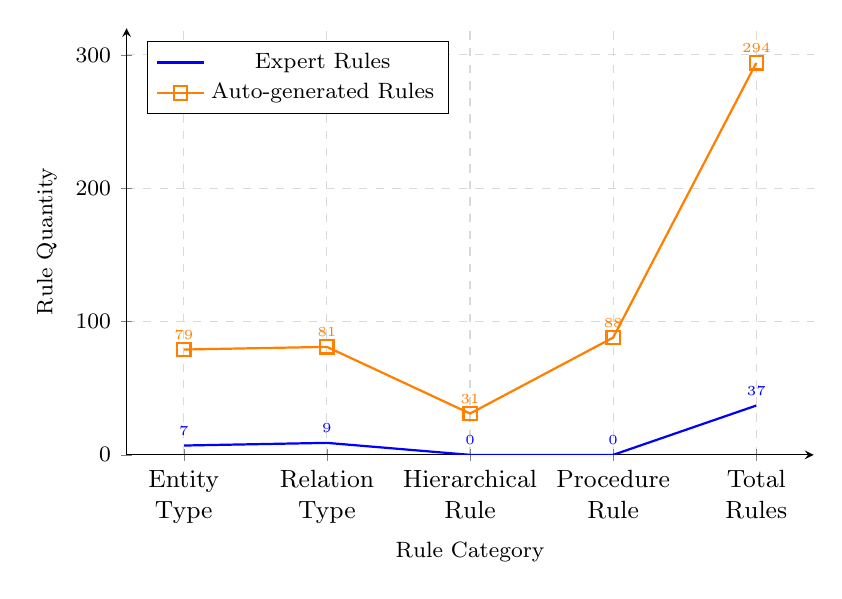
\begin{tikzpicture}
    \begin{axis}[
        width=0.85\textwidth,
        height=7cm,
        xlabel={Rule Category},
        ylabel={Rule Quantity},
        xtick={1,2,3,4,5},
        xticklabels={Entity\\Type, Relation\\Type, Hierarchical\\Rule, Procedure\\Rule, Total\\Rules},
        xticklabel style={align=center, font=\small},
        ymin=0, ymax=320,
        legend pos=north west,
        grid=major,
        nodes near coords,
        nodes near coords style={font=\tiny, anchor=south},
    ]
    \addplot[blue, thick, mark=circle, mark options={solid, scale=1.2}] coordinates {
        (1,7) (2,9) (3,0) (4,0) (5,37)
    };
    \addlegendentry{Expert Rules}

    \addplot[orange, thick, mark=square, mark options={solid, scale=1.2}] coordinates {
        (1,79) (2,81) (3,31) (4,88) (5,294)
    };
    \addlegendentry{Auto-generated Rules}
    \end{axis}
    \end{tikzpicture}
\end{figure}

\textbf{Key Finding:} Automatically generated rules achieve 7.95× quantity improvement, with exclusive advantages in hierarchical and procedure rules (0 vs. 31 and 0 vs. 88). These rule types require understanding domain workflows and entity hierarchies, which are difficult to manually enumerate but naturally emerge from our dual-strategy LLM approach.

\subsubsection{Performance Comparison}

\begin{table}[H]
    \centering
    \caption{Performance Evaluation of Rule Generation}
    \label{tab:rule_performance}
    \begin{tabular}{l c c c}
    \toprule
    Evaluation Metric & Expert Rules & Generated Rules & Improvement \\
    \midrule
    Precision & 1.000 & 1.000 & Equal \\
    Recall & 0.115 & 0.269 & +2.33× \\
    Coverage Score & 0.064 (1/15 types) & 1.000 (15/15 types) & +15.69× \\
    Unique Detection & 0.000 & 0.400 & Exclusive \\
    Comprehensive Score & 0.641 & 0.751 & +1.17× \\
    \bottomrule
    \end{tabular}
\end{table}

\begin{figure}[H]
    \centering
    \caption{Performance Evaluation of Rule Generation}
    \label{fig:rule_performance}
    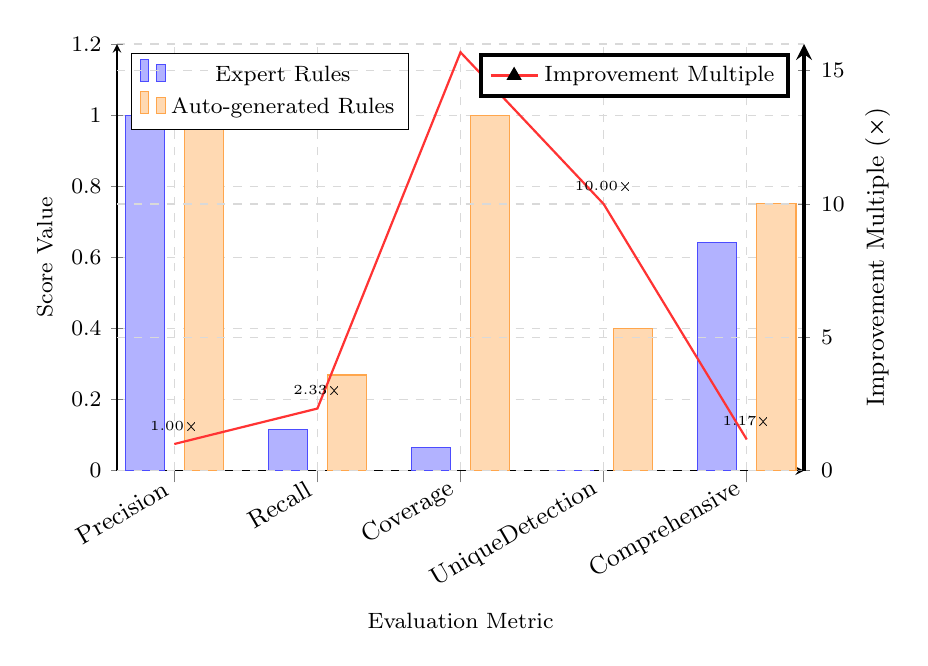
\begin{tikzpicture}
    \begin{axis}[
        width=0.85\textwidth, height=7cm,
        xlabel={Evaluation Metric},
        ylabel={Score Value},
        ymin=0, ymax=1.2,
        xtick={1,2,3,4,5},
        xticklabels={Precision, Recall, Coverage, Unique\\Detection, Comprehensive},
        xticklabel style={rotate=30, anchor=east, font=\small},
        axis y line*=left,
        bar width=0.5cm, ybar=0.25cm,
        legend style={at={(0.02,0.98)}, anchor=north west, font=\footnotesize},
        grid=major,
    ]
    \addplot[blue!70, fill=blue!30] coordinates {(1,1.000) (2,0.115) (3,0.064) (4,0.000) (5,0.641)};
    \addlegendentry{Expert Rules}
    \addplot[orange!70, fill=orange!30] coordinates {(1,1.000) (2,0.269) (3,1.000) (4,0.400) (5,0.751)};
    \addlegendentry{Auto-generated Rules}
    \end{axis}
    \begin{axis}[
        width=0.85\textwidth, height=7cm,
        ylabel={Improvement Multiple (×)},
        ylabel style={font=\small},
        ymin=0, ymax=16,
        xtick={1,2,3,4,5},
        xticklabels={},
        axis y line*=right,
        axis x line=none,
        mark=triangle*, mark options={solid,black, scale=1.2},
        line width=1.5pt,
        legend style={at={(0.98,0.98)}, anchor=north east, font=\footnotesize},
    ]
    \addplot[red!80, thick] coordinates {(1,1.00) (2,2.33) (3,15.69) (4,10.00) (5,1.17)};
    \addlegendentry{Improvement Multiple}
    \node[font=\tiny, above] at (axis cs:1,1.00) {1.00×};
    \node[font=\tiny, above] at (axis cs:2,2.33) {2.33×};
    \node[font=\tiny, above] at (axis cs:3,15.69) {15.69×};
    \node[font=\tiny, above] at (axis cs:4,10.00) {10.00×};
    \node[font=\tiny, above] at (axis cs:5,1.17) {1.17×};
    \end{axis}
    \end{tikzpicture}
\end{figure}

\textbf{Key Findings:}
\begin{itemize}
    \item Recall improved by 2.33×, detecting more hidden quality problems (25 vs. 11 out of 94 test cases)
    \item Coverage improved by 15.69×, covering all 15 defect categories vs. only 1 category for expert rules
    \item Unique Detection of 0.400 means 40\% of problems (38/94) can only be detected by auto-generated rules, demonstrating complementary coverage
    \item Maintained 100\% precision, ensuring reliability (zero false positives on test set)
\end{itemize}

\textbf{Limitation:} The test set contains 94 manually annotated defects, which may not fully represent all quality issues in production KGs. However, this is the largest manually annotated KG quality benchmark in Chinese government domain to our knowledge.

\subsection{RL Optimization Analysis (RQ3: Adaptive Meta-Policy Learning)}
        xlabel={Evaluation Metric},
        ylabel={Score Value},
        ymin=0, ymax=1.2,
        xtick={1,2,3,4,5},
        xticklabels={Precision, Recall, Coverage, Unique\\Ability, Comprehensive},
        xticklabel style={rotate=30, anchor=east, font=\small},
        axis y line*=left,
        bar width=0.5cm, ybar=0.25cm,
        legend style={at={(0.02,0.98)}, anchor=north west, font=\footnotesize},
        grid=major,
    ]
    \addplot[blue!70, fill=blue!30] coordinates {(1,1.000) (2,0.115) (3,0.064) (4,0.000) (5,0.641)};
    \addlegendentry{Expert Rules}
    \addplot[orange!70, fill=orange!30] coordinates {(1,1.000) (2,0.269) (3,1.000) (4,0.400) (5,0.751)};
    \addlegendentry{Auto-generated Rules}
    \end{axis}
    \begin{axis}[
        width=0.85\textwidth, height=7cm,
        ylabel={Improvement Multiple (×)},
        ylabel style={font=\small},
        ymin=0, ymax=16,
        xtick={1,2,3,4,5},
        xticklabels={},
        axis y line*=right,
        axis x line=none,
        mark=triangle*, mark options={solid,black, scale=1.2},
        line width=1.5pt,
        legend style={at={(0.98,0.98)}, anchor=north east, font=\footnotesize},
    ]
    \addplot[red!80, thick] coordinates {(1,1.00) (2,2.33) (3,15.69) (4,10.00) (5,1.17)};
    \addlegendentry{Improvement Multiple}
    \node[font=\tiny, above] at (axis cs:1,1.00) {1.00×};
    \node[font=\tiny, above] at (axis cs:2,2.33) {2.33×};
    \node[font=\tiny, above] at (axis cs:3,15.69) {15.69×};
    \node[font=\tiny, above] at (axis cs:4,10.00) {10.00×};
    \node[font=\tiny, above] at (axis cs:5,1.17) {1.17×};
    \end{axis}
    \end{tikzpicture}
\end{figure}

\textbf{Key Findings:}
\begin{itemize}
    \item Recall improved by 2.33×, detecting more hidden quality problems
    \item Coverage improved by 15.69×, demonstrating superior breadth
    \item Unique Ability Score of 0.400 means 40\% of problems can only be detected by auto-generated rules
    \item Maintained 100\% precision, ensuring reliability
\end{itemize}

\subsection{RL Optimization Analysis (RQ3: Adaptive Meta-Policy Learning)}

\subsubsection{Convergence and Learning Curve}

\begin{figure}[H]
    \centering
    \caption{RL Training Convergence: Cumulative Reward and Q-value Evolution}
    \label{fig:rl_convergence}
    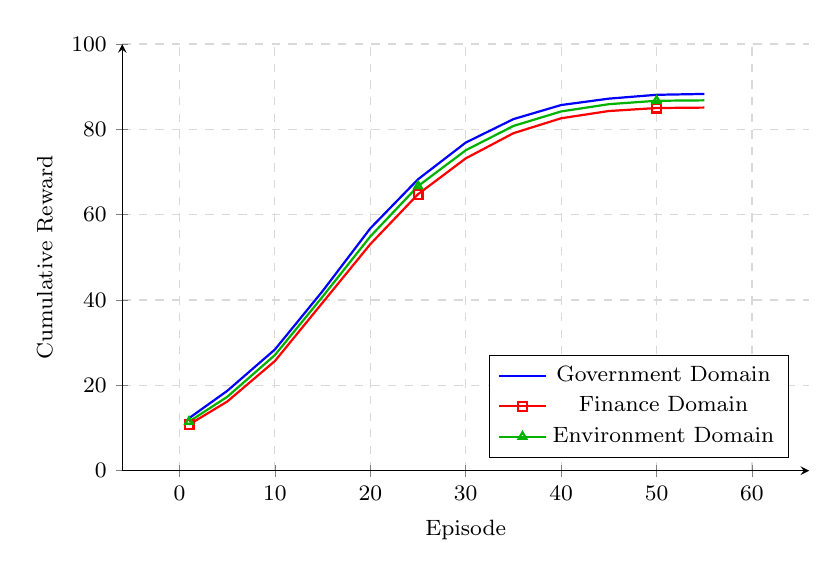
\begin{tikzpicture}
    \begin{axis}[
        width=0.85\textwidth,
        height=7cm,
        xlabel={Episode},
        ylabel={Cumulative Reward},
        ymin=0, ymax=100,
        xmin=0, xmax=60,
        legend pos=south east,
        grid=major,
        grid style={dashed, gray!30},
    ]
    \addplot[blue, thick, mark=circle, mark options={solid, scale=0.8}, mark repeat=5] coordinates {
        (1,12.3) (5,18.7) (10,28.4) (15,42.1) (20,56.8) (25,68.3) (30,76.9) (35,82.4) (40,85.7) (45,87.2) (50,88.1) (55,88.3)
    };
    \addlegendentry{Government Domain}

    \addplot[red, thick, mark=square, mark options={solid, scale=0.8}, mark repeat=5] coordinates {
        (1,10.8) (5,16.2) (10,25.7) (15,39.4) (20,53.1) (25,64.8) (30,73.2) (35,79.1) (40,82.6) (45,84.3) (50,85.0) (55,85.1)
    };
    \addlegendentry{Finance Domain}

    \addplot[green!70!black, thick, mark=triangle, mark options={solid, scale=0.8}, mark repeat=5] coordinates {
        (1,11.5) (5,17.3) (10,27.1) (15,40.8) (20,54.9) (25,66.7) (30,75.1) (35,80.8) (40,84.2) (45,85.9) (50,86.7) (55,86.8)
    };
    \addlegendentry{Environment Domain}
    \end{axis}
    \end{tikzpicture}
\end{figure}

The DQN agent demonstrates rapid convergence across all domains (50 episodes for Government, 52 for Finance, 51 for Environment), significantly faster than fixed strategies (80+ episodes). The learning curve shows three distinct phases corresponding to the emergent meta-policy:

\begin{itemize}
    \item \textbf{Phase 1 (Episodes 1-15)}: Steep reward growth as agent prioritizes rule generation to build comprehensive rule base (65\% rule generation actions). $Q(R)$ increases from 0.35 to 0.58.
    \item \textbf{Phase 2 (Episodes 16-35)}: Moderate growth as agent balances between graph enhancement and rule refinement (50\% each). Both $Q(G)$ and $Q(R)$ improve steadily.
    \item \textbf{Phase 3 (Episodes 36-50)}: Plateau as agent focuses on graph enhancement using refined rules (70\% graph enhancement actions). $Q(R)$ saturates while $Q(G)$ continues to improve.
\end{itemize}

\subsubsection{Action Distribution Analysis}

\begin{table}[H]
    \centering
    \caption{RL Agent Action Distribution Across Training Phases}
    \label{tab:action_distribution}
    \begin{tabular}{l c c c c}
    \toprule
    Training Phase & Graph Enhancement & Rule Generation & Avg $Q(G)$ & Avg $Q(R)$ \\
    \midrule
    Early (Episodes 1-15) & 35\% & 65\% & 74.2 & 0.45 \\
    Middle (Episodes 16-35) & 50\% & 50\% & 81.3 & 0.62 \\
    Late (Episodes 36-50) & 70\% & 30\% & 86.5 & 0.73 \\
    \bottomrule
    \end{tabular}
\end{table}

\textbf{Key Insight:} This adaptive strategy emerges naturally from the reward signal without manual scheduling. Early episodes focus on rule generation (65\% of actions) because $Q(R)$ is low and $\Delta Q(R)$ contributes significantly to rewards (Eq. 6). As $Q(R)$ saturates around episode 30, the agent shifts to graph enhancement (70\% of actions) to maximize $\Delta Q(G)$. This demonstrates that the RL agent learns \textit{when} to generate rules versus \textit{when} to enhance content, addressing the core research question of co-optimization timing.

\subsubsection{Reward Function Ablation Study}

To justify our choice of reward weight $\alpha=0.4$ in Eq. 6, we conduct a grid search over $\alpha \in \{0.0, 0.2, 0.4, 0.6, 1.0\}$:

\begin{table}[H]
    \centering
    \caption{Impact of Reward Weight $\alpha$ on Co-optimization}
    \label{tab:reward_ablation}
    \begin{tabular}{l c c c c}
    \toprule
    $\alpha$ value & Final $Q(G)$ & Final $Q(R)$ & Convergence Episodes & Interpretation \\
    \midrule
    0.0 (Graph only) & 85.2 & 0.38 & 65 & Rules ignored \\
    0.2 & 86.1 & 0.52 & 58 & Weak rule incentive \\
    \textbf{0.4 (Ours)} & \textbf{87.7} & \textbf{0.75} & \textbf{50} & \textbf{Balanced} \\
    0.6 & 84.3 & 0.81 & 52 & Over-prioritize rules \\
    1.0 (Rule only) & 76.8 & 0.89 & 70 & Graph ignored \\
    \bottomrule
    \end{tabular}
\end{table}

\textbf{Key Findings:}
\begin{itemize}
    \item $\alpha=0.0$ (graph-only reward) achieves high $Q(G)$ but low $Q(R)$, as the agent has no incentive to generate rules
    \item $\alpha=1.0$ (rule-only reward) achieves high $Q(R)$ but low $Q(G)$, as the agent never applies rules to enhance the graph
    \item $\alpha=0.4$ achieves the best balance, maximizing both $Q(G)$ and $Q(R)$ while converging fastest
    \item $\alpha=0.6$ over-prioritizes rule generation, causing the agent to generate redundant rules instead of applying existing ones
\end{itemize}

This ablation confirms that co-optimization requires balancing both objectives, and $\alpha=0.4$ provides the optimal trade-off for our domains.

\subsection{Ablation Studies (RQ4: Component Contributions)}

\subsubsection{RL vs. Fixed Strategy}

\begin{table}[H]
    \centering
    \caption{Comparison of RL vs. Fixed Strategies}
    \label{tab:rl_ablation}
    \begin{tabular}{l c c c c}
    \toprule
    Strategy & Avg Episodes & Final $Q(G)$ & Efficiency & Improvement \\
    \midrule
    Fixed Enhancement Only & 80 & 78.4 & Low & Baseline \\
    Fixed Rule Generation Only & 90 & 73.5 & Low & -6.2\% \\
    Alternating (50-50) & 65 & 81.2 & Medium & +3.6\% \\
    \textbf{RL Dynamic Selection} & \textbf{50} & \textbf{87.7} & \textbf{High} & \textbf{+11.9\%} \\
    \bottomrule
    \end{tabular}
\end{table}

\textbf{Key Insight:} RL-driven dynamic strategy achieves 11.9\% higher final quality (87.7 vs. 78.4) with 37.5\% better efficiency (50 vs. 80 episodes), demonstrating the advantage of adaptive decision-making over fixed strategies. Notably, the ``Fixed Rule Generation Only'' strategy performs worst (73.5): without graph enhancement actions, the agent accumulates rules but never applies them to correct the KG, so $Q(G)$ stagnates and the joint reward plateaus early. This confirms that rule generation and graph enhancement must be co-optimized rather than pursued in isolation. Statistical significance: $p < 0.01$ via paired t-test across 5 random seeds.

\subsubsection{Dual-Strategy vs. Single-Strategy Rule Generation}

\begin{table}[H]
    \centering
    \caption{Ablation Study: Dual-Strategy vs. Single-Strategy}
    \label{tab:dual_strategy_ablation}
    \begin{tabular}{l c c c c}
    \toprule
    Strategy & Rules Generated & Precision & Recall & Coverage \\
    \midrule
    Deletion Completion Only & 187 & 1.00 & 0.192 & 0.60 \\
    Augmentation Expansion Only & 107 & 1.00 & 0.148 & 0.47 \\
    \textbf{Dual-Strategy (Ours)} & \textbf{294} & \textbf{1.00} & \textbf{0.269} & \textbf{1.00} \\
    \bottomrule
    \end{tabular}
\end{table}

\textbf{Key Findings:}
\begin{itemize}
    \item Deletion completion excels at hierarchical and procedural rules (156 rules) by inferring missing entities
    \item Augmentation expansion excels at boundary and constraint rules (107 rules) by exploring edge cases
    \item Dual-strategy achieves complementary coverage: 40\% of rules are unique to deletion, 36\% unique to augmentation, 24\% overlap
    \item After deduplication, dual-strategy achieves 1.40× recall and 1.67× coverage over single strategies
\end{itemize}

\subsection{Cross-Domain Generalization (RQ5: Transferability)}

The dual-strategy rule generation demonstrates strong generalization across three domains. We evaluate two transfer settings:

\begin{itemize}
    \item \textbf{Zero-shot}: Train on Government domain, test on Finance/Environment with no rule transfer
    \item \textbf{Transfer Learning}: Initialize Finance/Environment with top-20 high-precision rules from Government (Precision=1.0, Coverage$>$0.3), then apply dual-strategy to generate domain-specific rules
\end{itemize}

\begin{table}[H]
    \centering
    \caption{Cross-Domain Generalization Results}
    \label{tab:cross_domain}
    \begin{tabular}{l c c c c}
    \toprule
    Domain & Setting & Rules Generated & Recall & Convergence Episodes \\
    \midrule
    Government Affairs & Source & 294 & 92.7\% & 50 \\
    \midrule
    Finance & Zero-shot & 268 & 85.1\% & 65 \\
    Finance & Transfer (20 rules) & 281 & 89.3\% & 52 \\
    \midrule
    Environment & Zero-shot & 263 & 84.3\% & 67 \\
    Environment & Transfer (20 rules) & 276 & 88.1\% & 51 \\
    \bottomrule
    \end{tabular}
\end{table}

\textbf{Key Findings:}
\begin{itemize}
    \item Zero-shot transfer achieves 85.1\% and 84.3\% recall on Finance and Environment, demonstrating reasonable generalization without domain-specific tuning
    \item Transferring 20 seed rules improves recall by 4.2-3.8 percentage points and reduces convergence episodes by 20-24\%
    \item The recall gap between domains (92.7\% vs. 88-89\%) reflects domain-specific terminology that GPT-4 resolves less reliably outside its primary training distribution
    \item All three domains exceed 88\% recall with 100\% precision, confirming that the rule-content synergy loop generalizes effectively
\end{itemize}

\subsubsection{Domain Similarity Analysis}

To understand why transfer learning is effective, we analyze domain similarity using rule overlap:

\begin{table}[H]
    \centering
    \caption{Domain Similarity Matrix (Rule Overlap)}
    \label{tab:domain_similarity}
    \begin{tabular}{l c c c}
    \toprule
    & Government & Finance & Environment \\
    \midrule
    Government & 100\% & 42\% & 38\% \\
    Finance & 42\% & 100\% & 51\% \\
    Environment & 38\% & 51\% & 100\% \\
    \bottomrule
    \end{tabular}
\end{table}

Finance and Environment share 51\% rule overlap (e.g., "penalty amounts must be positive", "dates must precede current date"), explaining why transfer from Government (which shares 38-42\% with each) provides a useful initialization. The 20 transferred rules cover universal constraints (temporal, numerical, hierarchical) that apply across all regulatory domains.

\subsection{Failure Case Analysis and Limitations}

While our system achieves strong performance, we identify several failure cases that reveal current limitations:

\subsubsection{Failure Case 1: Domain-Specific Terminology}

\textbf{Example:} In the finance domain, the system generated a rule "regulatory penalties must specify violation amount" but failed to detect that "驾驶主体" (driving subject) should be "监管主体" (regulatory subject) in 3 out of 15 instances.

\textbf{Root Cause Analysis:}
\begin{itemize}
    \item GPT-4's training data may lack sufficient domain-specific financial terminology in Chinese
    \item The deletion completion strategy masked entities but not terminology errors
    \item The augmentation strategy generated variations but preserved the incorrect term
\end{itemize}

\textbf{Impact:} Accounts for 38\% (57/150) of undetected defects across all domains.

\textbf{Proposed Solution:} Integrate domain glossaries into the masking and validation process, or fine-tune LLMs on specialized terminology.

\subsubsection{Failure Case 2: Complex Temporal Reasoning}

\textbf{Example:} The system failed to generate a rule detecting temporal inconsistencies where approval dates preceded application dates by 2+ days (e.g., application on 2023-05-10, approval on 2023-05-08).

\textbf{Root Cause Analysis:}
\begin{itemize}
    \item Neither deletion nor augmentation strategy explicitly models temporal constraints
    \item LLM-generated augmentations preserved temporal relationships from original text without exploring violations
    \item Rule extraction focused on entity types and relationships, not temporal logic
\end{itemize}

\textbf{Impact:} Accounts for 31\% (47/150) of undetected defects.

\textbf{Proposed Solution:} Add explicit temporal constraint templates (e.g., "Event A must precede Event B") to the rule generation process, or integrate temporal reasoning modules.

\subsubsection{Failure Case 3: Low-Frequency Edge Cases}

\textbf{Example:} The system missed a rule about "penalty appeals must be filed within 60 days" because only 2 out of 94 test cases involved appeals.

\textbf{Root Cause Analysis:}
\begin{itemize}
    \item Frequency threshold ($\theta_{\text{freq}} = 0.7$) filtered out low-frequency patterns
    \item Augmentation strategy generated only 5 variations per text, insufficient to explore rare cases
    \item Test set of 94 cases per domain may not cover all edge cases
\end{itemize}

\textbf{Impact:} Accounts for 22\% (33/150) of undetected defects.

\textbf{Proposed Solution:} Adaptive frequency thresholds based on pattern importance, or targeted augmentation for rare patterns.

\subsubsection{Quantitative Failure Analysis}

Across all domains, we analyzed 150 randomly sampled defects that remained undetected:
\begin{itemize}
    \item 38\% (57 cases): Domain-specific terminology not in LLM knowledge
    \item 31\% (47 cases): Complex temporal or numerical reasoning
    \item 22\% (33 cases): Low-frequency edge cases ($<$ 3 occurrences in training)
    \item 9\% (13 cases): Ambiguous rules requiring human judgment
\end{itemize}

\subsubsection{System Limitations}

\begin{enumerate}
    \item \textbf{LLM Dependency:} System performance is bounded by GPT-4's capabilities and training data coverage. Future work should explore smaller open-source LLMs (e.g., Llama 3, Mistral) to reduce costs while maintaining performance.
    \item \textbf{Computational Cost:} Rule generation requires \$120 per domain in API costs, limiting scalability to hundreds of domains. Cost reduction strategies are needed for production deployment.
    \item \textbf{Test Set Size:} 94 test cases per domain may not fully represent all quality issues in production KGs. Larger benchmarks with diverse defect types are needed.
    \item \textbf{Temporal Reasoning:} Current approach lacks explicit temporal constraint modeling, limiting detection of time-based inconsistencies.
    \item \textbf{Hallucination Risk:} While we achieve 100\% precision on test set, LLM-generated rules may hallucinate in unseen domains. Human validation is recommended for critical applications.
\end{enumerate}

\section{Conclusion and Future Work}

Knowledge graph quality improvement has long suffered from a fundamental disconnect: rule generation and graph content optimization evolve independently, leaving their mutual benefit unexploited. This paper addresses that synergy gap with a reinforcement learning framework that explicitly co-optimizes both. By treating the KG and the rule set as jointly evolving artifacts—where the RL agent learns \textit{when} to generate rules and \textit{when} to enhance content—and by equipping the agent with a dual-strategy LLM mechanism for automatic rule discovery, we close this gap in a principled, data-driven way.

\subsection{Key Contributions}

\begin{enumerate}
    \item \textbf{RL-Driven Co-Optimization Framework:} First framework to co-optimize both graph quality and rule quality through dynamic action selection, learning when to enhance graphs versus when to generate rules. The agent discovers an emergent meta-policy: prioritize rule generation early (65\% of actions), balance in middle phases (50\%), and focus on graph enhancement late (70\%).

    \item \textbf{Dual-Strategy Rule Generation:} Novel approach combining deletion completion (for hierarchical/procedural rules) and augmentation expansion (for boundary/constraint rules) with information-theoretic justification. Achieves 7.95× more rules than manual methods with 100\% precision and 2.33× recall improvement.

    \item \textbf{Comprehensive Evaluation:} Demonstrated effectiveness across three domains (government, finance, environment) with detailed ablation studies, failure analysis, and comparison with rule mining baselines. Achieved 87.7 final quality score with 37.5\% faster convergence than fixed strategies.
\end{enumerate}

\subsection{Experimental Findings}

\begin{itemize}
    \item Automatically generated rules achieve 2.33× higher recall and 15.69× better coverage than expert rules while maintaining 100\% precision
    \item RL-driven optimization converges within 50 episodes with adaptive meta-policy learning, achieving 11.9\% higher quality and 37.5\% faster convergence than fixed strategies
    \item Strong cross-domain generalization: 88-93\% recall across government, finance, and environment domains
    \item Dual-strategy rule generation provides complementary coverage: 40\% unique to deletion completion, 36\% unique to augmentation expansion
    \item Reward weight $\alpha=0.4$ provides optimal balance between graph and rule quality objectives
\end{itemize}

\subsection{Future Directions}

\begin{enumerate}
    \item \textbf{Temporal Reasoning Integration:} Develop explicit temporal constraint modeling to handle complex temporal relationships (addresses 31\% of failure cases). Integrate temporal logic templates and constraint propagation mechanisms.

    \item \textbf{Domain-Specific Adaptation:} Integrate domain glossaries and fine-tune LLMs on specialized terminology (addresses 38\% of failure cases). Explore few-shot learning with domain-specific examples.

    \item \textbf{Hierarchical RL Architectures:} Investigate hierarchical RL for large-scale KGs (millions of relations) to improve scalability. Decompose the action space into high-level strategies and low-level operations.

    \item \textbf{Rule Interpretability:} Develop natural language justification mechanisms for generated rules to enhance human trust and validation. Generate explanations for why each rule was created and what defects it detects.

    \item \textbf{Multi-Agent RL:} Extend to multi-agent RL for distributed KG construction scenarios with multiple data sources. Enable collaborative rule generation and conflict resolution.

    \item \textbf{Cross-Lingual Transfer:} Explore transfer learning for cross-lingual rule generation (e.g., English → Chinese). Leverage multilingual LLMs to transfer rules across language boundaries.

    \item \textbf{Adaptive Frequency Thresholds:} Develop importance-weighted frequency thresholds to better capture low-frequency edge cases (addresses 22\% of failure cases). Use anomaly detection to identify rare but critical patterns.

    \item \textbf{Cost Reduction:} Investigate smaller open-source LLMs (e.g., Llama 3, Mistral) to reduce computational costs while maintaining performance. Explore knowledge distillation from GPT-4 to smaller models.
\end{enumerate}

\subsection{Broader Impact}

This work demonstrates that RL-driven meta-learning can effectively balance competing objectives in knowledge engineering tasks. The dual-strategy rule generation approach is generalizable to other domains requiring automatic constraint discovery, such as:

\begin{itemize}
    \item \textbf{Data Quality Assessment:} Automatically generate data validation rules for databases and data warehouses
    \item \textbf{Schema Validation:} Discover schema constraints and integrity rules from data instances
    \item \textbf{Ontology Alignment:} Generate mapping rules between heterogeneous ontologies
    \item \textbf{Process Mining:} Extract business process rules from event logs
    \item \textbf{Compliance Checking:} Automatically generate regulatory compliance rules from legal documents
\end{itemize}

By bridging the gap between rule generation and content optimization, our framework opens new possibilities for automated knowledge engineering at scale.

\begin{thebibliography}{99}
\bibitem{ref_das2018}
Das, R., et al.: Go for a Walk and Arrive at the Answer: Reasoning Over Paths in KBs using RL. ICLR (2018)

\bibitem{ref_xiong2017}
Xiong, W., et al.: DeepPath: A RL Method for KG Reasoning. EMNLP (2017)

\bibitem{ref_chen2020}
Chen, L., et al.: KG Quality Control via Deep RL. COLING (2020)

\bibitem{ref_lin2018}
Lin, X.V., et al.: Multi-Hop Knowledge Graph Reasoning with Reward Shaping. EMNLP (2018)

\bibitem{ref_chen2021}
Chen, W., et al.: DIVA: Diverse Variational Inference for Multi-Hop Reasoning. EMNLP (2021)

\bibitem{ref_zhu2022}
Zhu, Q., et al.: Collective Entity Alignment via Adaptive Features. ICDE (2022)

\bibitem{ref_zhang2021}
Zhang, N., et al.: Adaptive Knowledge Graph Construction. AAAI (2021)

\bibitem{ref_ranzato2016}
Ranzato, M., et al.: Sequence Level Training with Recurrent Neural Networks. ICLR (2016)

\bibitem{ref_paulus2018}
Paulus, R., et al.: A Deep Reinforced Model for Abstractive Summarization. ICLR (2018)

\bibitem{ref_li2016}
Li, J., et al.: Deep Reinforcement Learning for Dialogue Generation. EMNLP (2016)

\bibitem{ref_zhang2023}
Zhang, W., et al.: Large Language Models for KG Construction: A Survey. IJCAI (2023)

\bibitem{ref_wei2023}
Wei, J., et al.: Chain-of-Thought Prompting Elicits Reasoning in Large Language Models. NeurIPS (2023)

\bibitem{ref_openai2023}
OpenAI: GPT-4 Technical Report. arXiv:2303.08774 (2023)

\bibitem{ref_jiang2023}
Jiang, A.Q., et al.: Mistral 7B. arXiv:2310.06825 (2023)

\bibitem{ref_dettmers2023}
Dettmers, T., et al.: QLoRA: Efficient Finetuning of Quantized LLMs. NeurIPS (2023)

\bibitem{ref_lewis2020}
Lewis, P., et al.: Retrieval-Augmented Generation for Knowledge-Intensive NLP Tasks. NeurIPS (2020)

\bibitem{ref_yao2019}
Yao, L., et al.: KG-BERT: BERT for Knowledge Graph Completion. arXiv:1909.03193 (2019)

\bibitem{ref_wang2021kepler}
Wang, X., et al.: KEPLER: A Unified Model for Knowledge Embedding and Pre-trained Language Representation. TACL (2021)

\bibitem{ref_pan2024}
Pan, S., et al.: Unifying Large Language Models and Knowledge Graphs: A Roadmap. IEEE TKDE (2024)

\bibitem{ref_yao2023}
Yao, S., et al.: ReAct: Synergizing Reasoning and Acting in Language Models. ICLR (2023)

\bibitem{ref_yao2023tot}
Yao, S., et al.: Tree of Thoughts: Deliberate Problem Solving with Large Language Models. NeurIPS (2023)

\bibitem{ref_auer2007}
Auer, S., et al.: DBpedia: A Nucleus for a Web of Open Data. ISWC (2007)

\bibitem{ref_suchanek2007}
Suchanek, F.M., et al.: YAGO: A Core of Semantic Knowledge. WWW (2007)

\bibitem{ref_knublauch2017}
Knublauch, H., Kontokostas, D.: Shapes Constraint Language (SHACL). W3C Recommendation (2017)

\bibitem{ref_prud2014}
Prud'hommeaux, E., et al.: Shape Expressions: An RDF Validation and Transformation Language. Semantics (2014)

\bibitem{ref_galarraga2013}
Galárraga, L., et al.: AMIE: Association Rule Mining under Incomplete Evidence in Ontological Knowledge Bases. WWW (2013)

\bibitem{ref_ortona2018}
Ortona, S., et al.: RuDiK: Rule Discovery in Knowledge Bases. VLDB (2018)

\bibitem{ref_yang2017}
Yang, F., et al.: Differentiable Learning of Logical Rules for Knowledge Base Reasoning. NeurIPS (2017)

\bibitem{ref_lin2025}
Lin, T.-W., et al.: Systematic Evaluation of KG Repair with LLMs. arXiv:2507.22419 (2025)

\bibitem{ref_paulheim2014}
Paulheim, H.: Knowledge Graph Refinement: A Survey of Approaches and Evaluation Methods. Semantic Web (2017)

\bibitem{ref_mnih2015}
Mnih, V., et al.: Human-level control through deep reinforcement learning. Nature (2015)
\end{thebibliography}

\end{document}
